\documentclass[12pt]{article}
 
\usepackage[margin=1in]{geometry} 
\usepackage{amsmath,amsthm,amssymb}
\usepackage{hyperref}
\usepackage{graphicx}
\usepackage{xcolor}
\usepackage[many]{tcolorbox}
\tcbuselibrary{listings}
\usepackage{listings}
%jari:
\usepackage{enumitem}

\definecolor{lg}{HTML}{f0f0f0}

\newtcblisting{pycode}{
    colback=lg,
    boxrule=0pt,
    arc=0pt,
    outer arc=0pt,
    top=0pt,
    bottom=0pt,
    colframe=white,
    listing only,
    left=15.5pt,
    enhanced,
    listing options={
        basicstyle=\small\ttfamily,
        keywordstyle=\color{blue},
        language=Python,
        showstringspaces=false,
        tabsize=2,
        numbers=left,
        breaklines=true
    },
    overlay={
        \fill[gray!30]
        ([xshift=-3pt]frame.south west)
        rectangle
        ([xshift=11.5pt]frame.north west);
    }
}

\lstset{
    language=Python,
    basicstyle=\small\ttfamily,
}

 
\begin{document}
 
\title{Exercise 4}
\author{Jari Mattila - 35260T\\
ELEC-E8125 - Reinforcement Learning}

\maketitle

\section*{Task 1}

The training performance plots are presented below for Task 1a using 
handcrafted feature vector $\phi(s) = [s,|s|]^T$ in Figure~\ref*{fig:fig1} and Task 1b 
using radial basis function representations in Figure~\ref*{fig:fig2}.
\newline

\begin{figure}[h] 
	\centering  % Remember to centre the figure
    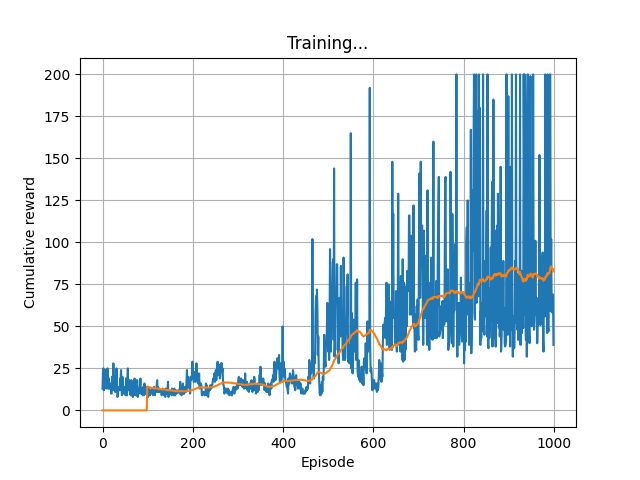
\includegraphics[width=0.9\columnwidth]{img/Figure_1_task_1a_cumulative_reward.png}
	\caption{Training performance using handcrafted feature vector $\phi(s) = [s,|s|]^T$.}
	\label{fig:fig1}
\end{figure}

\begin{figure}[h] 
	\centering  % Remember to centre the figure
    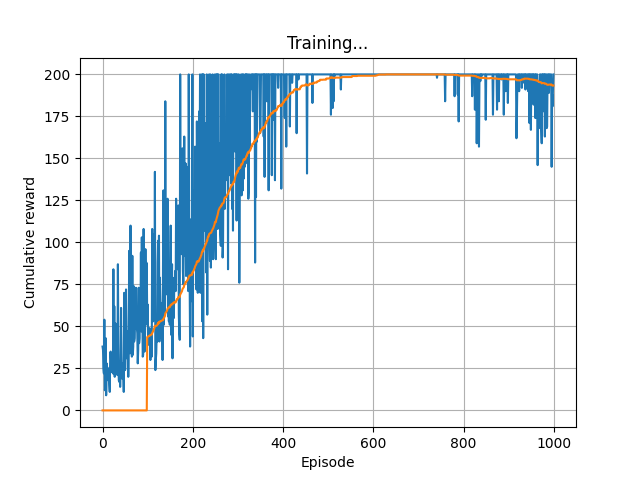
\includegraphics[width=0.9\columnwidth]{img/Figure_2_task_1b_cumulative_reward.png}
	\caption{Training performance using radial basis function representations.}
	\label{fig:fig2}
\end{figure}

\noindent
Source files: main\_task1.py, rbf\_agent\_task1a.py, rbf\_agent\_task1b.py 


\section*{Question 1}

Would it be possible to learn accurately Q-values for the Cartpole
problem using linear features (by passing the state directly to a linear regressor)? Why/why
not?
\newline

Learning Q-values for the Cartpole problem accurately using linear features can be difficult because the linear model cannot model dependencies between the features.
\newline

For example, in the Cartpole problem the high angular velocity can be either good or bad depending on the angle - this cannot be taken into account by the linear model (for details see Section 9.5 of Sutton's book).
\newline

and use~\cite{sutton2018reinforcement}.

\pagebreak


\section*{Task 2}

Modify your Task 1 implementation to perform minibatch updates and
use experience replay (\textbf{while keeping the original code for Task 1 submission}) [1, p. 440].
Run the experiments with Cartpole with both feature representations.
\newline

Training plots of all methods (Task 1 a), b), Task 2 and Task 4).
\newline

\noindent
Source files: main\_task1.py, rbf\_agent\_task1a.py, rbf\_agent\_task1b.py 

\section*{Question 2}

Figure 2 shows the training performance of all four methods from Task 1, together
with grid-based learning from Exercise 3 evaluated using GLIE with a = 50.

\section*{Question 2.1}

How does the experience replay affect the learning performance?

\section*{Question 2.2}

Discuss the benefits and cons of using hand-crafted features. As an example, you can refer to 
the given hand-crafted feature and more complex features like
$\phi(s) = [s_x, s_{\dot{x}}, \operatorname{cos}(s_{\theta}), \operatorname{sin}(s_{\theta}), s_{\dot{\theta}}]^T$

\section*{Question 2.3}

Do grid based methods look sample-efficient compared to any of the
function approximation methods? Why/why not?

\section*{Task 3}

Create a 2D plot of policy (best action in terms of state) learned with RBF
with experience replay in terms of $x$ and $\theta$ for $\dot{x}=0$ and $\dot{\theta}=0$.
\newline

Policy plot from Task 3.
\newline

\noindent
Source files: qlearning.py, xx.py 

\section*{Task 4}

Replace the RBFs in your Task 2 implementation with a neural network
(\textbf{while keeping the original code for Task 2 submission}). A basic DQN implementation
can be found in dqn\_agent.py. Evaluate the method’s performance in CartPole and LunarLander
environments.
\newline

Training plots of all methods (Task 1 a), b), Task 2 and Task 4).
\newline

\noindent
Source files: qlearning.py, xx.py 

\section*{Question 3.1}

Can Q-learning be used directly in environments with continuous
action spaces?

\section*{Question 3.2}

Which steps of the algorithm would be difficult to compute in case of
a continuous action space? If any, what could be done to solve them?


\pagebreak



\bibliographystyle{ieeetr}
\bibliography{template}  % Modify template with your bibliography name
\end{document}
